\documentclass{article}
\usepackage{tikz}
\usetikzlibrary{calc,scopes}

\begin{document}

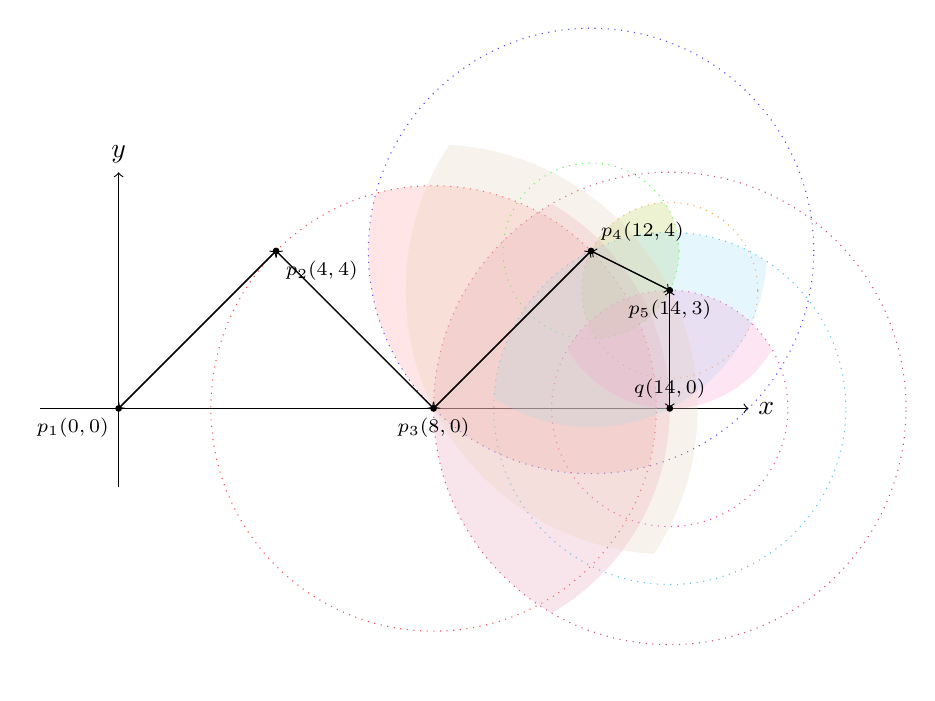
\begin{tikzpicture}[scale=0.5]
    % Define coordinates
    \coordinate (p1) at (0,0);
    \coordinate (p2) at (4,4);
    \coordinate (p3) at (8,0);
    \coordinate (p4) at (12,4);
    \coordinate (p5) at (14,3);
    \coordinate (q) at (14,0);

    % Draw axes
    \draw[->] (-2,0) -- (16,0) node[right] {$x$};
    \draw[->] (0,-2) -- (0,6) node[above] {$y$};

    % Draw all circles as before, but with slightly darker, soft boundaries
    \draw[red!70, dotted, thin] let \p1=(p3), \p2=(p4), \n1={veclen(\x2-\x1,\y2-\y1)} in (p3) circle (\n1);
    \draw[blue!70, dotted, thin] let \p1=(p4), \p2=(p3), \n1={veclen(\x2-\x1,\y2-\y1)} in (p4) circle (\n1);
    \draw[green!70, dotted, thin] let \p1=(p4), \p2=(p5), \n1={veclen(\x2-\x1,\y2-\y1)} in (p4) circle (\n1);
    \draw[orange!70, dotted, thin] let \p1=(p5), \p2=(p4), \n1={veclen(\x2-\x1,\y2-\y1)} in (p5) circle (\n1);
    % Draw the new circles for q
    \draw[purple!70, dotted, thin] let \p1=(q), \p2=(p3), \n1={veclen(\x2-\x1,\y2-\y1)} in (q) circle (\n1);
    \draw[cyan!70, dotted, thin] let \p1=(q), \p2=(p4), \n1={veclen(\x2-\x1,\y2-\y1)} in (q) circle (\n1);
    \draw[magenta!70, dotted, thin] let \p1=(q), \p2=(p5), \n1={veclen(\x2-\x1,\y2-\y1)} in (q) circle (\n1);

    % Update all lune fills to be a bit darker
    % Lune between circle centered at p3 and p4 (excluding overlap with p5)
    \begin{scope}
        \clip let \p1=(p3), \p2=(p4), \n1={veclen(\x2-\x1,\y2-\y1)} in (p3) circle (\n1);
        \path[fill=red!40, fill opacity=0.25, draw=none] let \p1=(p4), \p2=(p3), \n1={veclen(\x2-\x1,\y2-\y1)} in (p4) circle (\n1);
    \end{scope}
    % Lune between circle centered at p4 and p5 (excluding overlap with p3)
    \begin{scope}
        \clip let \p1=(p4), \p2=(p5), \n1={veclen(\x2-\x1,\y2-\y1)} in (p4) circle (\n1);
        \path[fill=green!40, fill opacity=0.25, draw=none] let \p1=(p5), \p2=(p4), \n1={veclen(\x2-\x1,\y2-\y1)} in (p5) circle (\n1);
    \end{scope}
    % Lune between circle centered at p5 and p4 (excluding overlap with p3)
    \begin{scope}
        \clip let \p1=(p5), \p2=(p4), \n1={veclen(\x2-\x1,\y2-\y1)} in (p5) circle (\n1);
        \path[fill=orange!40, fill opacity=0.25, draw=none] let \p1=(p4), \p2=(p5), \n1={veclen(\x2-\x1,\y2-\y1)} in (p4) circle (\n1);
    \end{scope}
    % Lune between circle centered at q and p3
    \begin{scope}
        \clip let \p1=(q), \p2=(p3), \n1={veclen(\x2-\x1,\y2-\y1)} in (q) circle (\n1);
        \path[fill=purple!40, fill opacity=0.25, draw=none] let \p1=(p3), \p2=(q), \n1={veclen(\x2-\x1,\y2-\y1)} in (p3) circle (\n1);
    \end{scope}
    % Lune between circle centered at q and p4
    \begin{scope}
        \clip let \p1=(q), \p2=(p4), \n1={veclen(\x2-\x1,\y2-\y1)} in (q) circle (\n1);
        \path[fill=cyan!40, fill opacity=0.25, draw=none] let \p1=(p4), \p2=(q), \n1={veclen(\x2-\x1,\y2-\y1)} in (p4) circle (\n1);
    \end{scope}
    % Lune between circle centered at q and p5
    \begin{scope}
        \clip let \p1=(q), \p2=(p5), \n1={veclen(\x2-\x1,\y2-\y1)} in (q) circle (\n1);
        \path[fill=magenta!40, fill opacity=0.25, draw=none] let \p1=(p5), \p2=(q), \n1={veclen(\x2-\x1,\y2-\y1)} in (p5) circle (\n1);
    \end{scope}
    % Lune between circle centered at p3 and p5
    \begin{scope}
        \clip let \p1=(p3), \p2=(p5), \n1={veclen(\x2-\x1,\y2-\y1)} in (p3) circle (\n1);
        \path[fill=brown!40, fill opacity=0.25, draw=none] let \p1=(p5), \p2=(p3), \n1={veclen(\x2-\x1,\y2-\y1)} in (p5) circle (\n1);
    \end{scope}

    % Draw directed edges on top of circles/shadings, but below points
    \draw[->, thin] (p1) -- (p2);
    \draw[->, thin] (p2) -- (p1);
    \draw[->, thin] (p2) -- (p3);
    \draw[->, thin] (p3) -- (p2);
    \draw[->, thin] (p3) -- (p4);
    \draw[->, thin] (p4) -- (p3);
    \draw[->, thin] (p4) -- (p5);
    \draw[->, thin] (p5) -- (p4);
    \draw[->, thin] (p5) -- (q);
    \draw[->, thin] (q) -- (p5);

    % Draw points on top of everything else, with smaller coordinate labels
    \filldraw (p1) circle (2pt) node[below left] {\scriptsize $p_1(0,0)$};
    \filldraw (p2) circle (2pt) node[below right] {\scriptsize $p_2(4,4)$};
    \filldraw (p3) circle (2pt) node[below] {\scriptsize $p_3(8,0)$};
    \filldraw (p4) circle (2pt) node[above right] {\scriptsize $p_4(12,4)$};
    \filldraw (p5) circle (2pt) node[below] {\scriptsize $p_5(14,3)$};
    \filldraw (q) circle (2pt) node[above] {\scriptsize $q(14,0)$};

\end{tikzpicture}

\end{document}
